\documentclass[11pt,a4paper]{article}

\onecolumn

\usepackage{ucs}
\usepackage[utf8x]{inputenc}
\usepackage[T1]{fontenc}
\usepackage[ngerman]{babel}
\usepackage{multibib}
\usepackage{hyperref}
\usepackage{Seminararbeit-Vorlage/seminararbeit-vorlage}

\usepackage[nottoc,numbib]{tocbibind}

% Use Helvet font globally
\usepackage{helvet}
\renewcommand{\familydefault}{\sfdefault}

% Set distance between two lines
\usepackage{setspace}
\onehalfspacing

% Indent the first line of a paragraph
\usepackage{indentfirst}

% Set margins
\usepackage{geometry}
\geometry{verbose,a4paper,tmargin=25mm,bmargin=25mm,lmargin=30mm,rmargin=30mm}

% Print the page number on the center head
\usepackage{scrpage2} 
\clearscrheadfoot 
\chead{-\ \pagemark\ -} 
\pagestyle{scrheadings} 

% Start document

\begin{document}

% Frontpage
\title{Transparente Kunststoffe in der Informationstechnologie}
\author{Tobias Schmidt}
\school{RUDOLF-DIESEL-GYMNASIUM AUGSBURG}
\year{2014/2016}
\subject{Chemie}
\seminar{Kunststoffchemie}
\supervisor{Fr. Müllerburger}
\deadline{10.11.2015}
\genderAppendixAuthor{}
\genderAppendixSupervisor{in}
\maketitle

\include{./Inhaltsverzeichnis}

\section{Speicherung und Weitergabe von Informationen im historischen Kontext}
\label{sec:einleitung}

Informationen speichern und weitergeben ist zentraler Bestandteil der
menschlichen Kultur und führte in der Menschheitsgeschichte zu bahnbrechenden
Erfindungen und laufenden Innovationen.

In der Steinzeit wurden Informationen an Höhlenwände gemalt, ab dem
\nolbreaks{3. Jahrtausend} vor Christus mittels Keilschrift (siehe
\autoref{fig:keilschrift}) in Steintafeln gemeißelt und in der Antike auf
Papyrus gezeichnet. Mitte des \nolbreaks{15. Jahrhunderts} revolutionierte
Gutenberg die Informationsweitergabe mit der Erfindung des Buchdrucks, der die
Produktion von Büchern in hohen Stückzahlen und zu geringen Kosten ermöglichte.
Auch heute noch wird diese Technik für die Reproduktion von Texten verwendet.

Ende des \nolbreaks{19. Jahrhunderts} gelang es erstmals, Musik zu speichern und
abzuspielen. Hierfür wurden zunächst Musikwalzen eingesetzt. Diese wurden um
1900 dann von Schallplatten aus einer Pressmasse aus Schellack\footnote{harzige
Ausscheidung von Lackschildläusen \cite{schellack}} (siehe
\autoref{fig:schallplatte-schellack}) abgelöst. Auf Schellackplatten konnten
Musikstücke mit bis zu fünf Minuten Spielzeit gespeichert werden und wurden auf
einem Grammophon abgespielt. Mit dem Einsatz des Kunststoffes Polyvinylchlorid
ab den 50er Jahren des \nolbreaks{20. Jahrhunderts} verbesserte sich die
Tonqualität von Schallplatten deutlich. Außerdem konnten längere Stücke
gespeichert und wiedergegeben werden. \cite{schallplatte1}

Mit der Compact Cassette (CC bzw. MC, siehe \autoref{fig:compact-cassette}), die
1963 auf den Markt kam, war es dann jedem möglich, selbst Musik aufzunehmen und
dauerhaft zu speichern \cite{kassette}. Compact Cassetten verwenden ein
Magnetband, das aus einer langen schmalen Kunststofffolie besteht, die mit einem
magnetisierbaren Material beschichtet wurde \cite{tonband}.

\ifthenelse{\boolean{showPics}}{
    \begin{figure}[h]
        \begin{center}
            \begin{minipage}[t]{0.3\textwidth}
                \begin{center}
                    \includegraphics[height=0.1\textheight]{Bilder/Einleitung/keilschrift.png}
                    \caption[Altpersische Keilschrift \newline \url{http://www.faz.net/aktuell/feuilleton/geisteswissenschaften/keilschriften-zehntausend-freunde-mesopotamiens-1657070.html} (zuletzt aufgerufen am 19.09.2015)]{Altpersische Keilschrift}
                    \label{fig:keilschrift}
                \end{center}
            \end{minipage}
            \hspace{0.025\textwidth}
            \begin{minipage}[t]{0.3\textwidth}
                \begin{center}
                    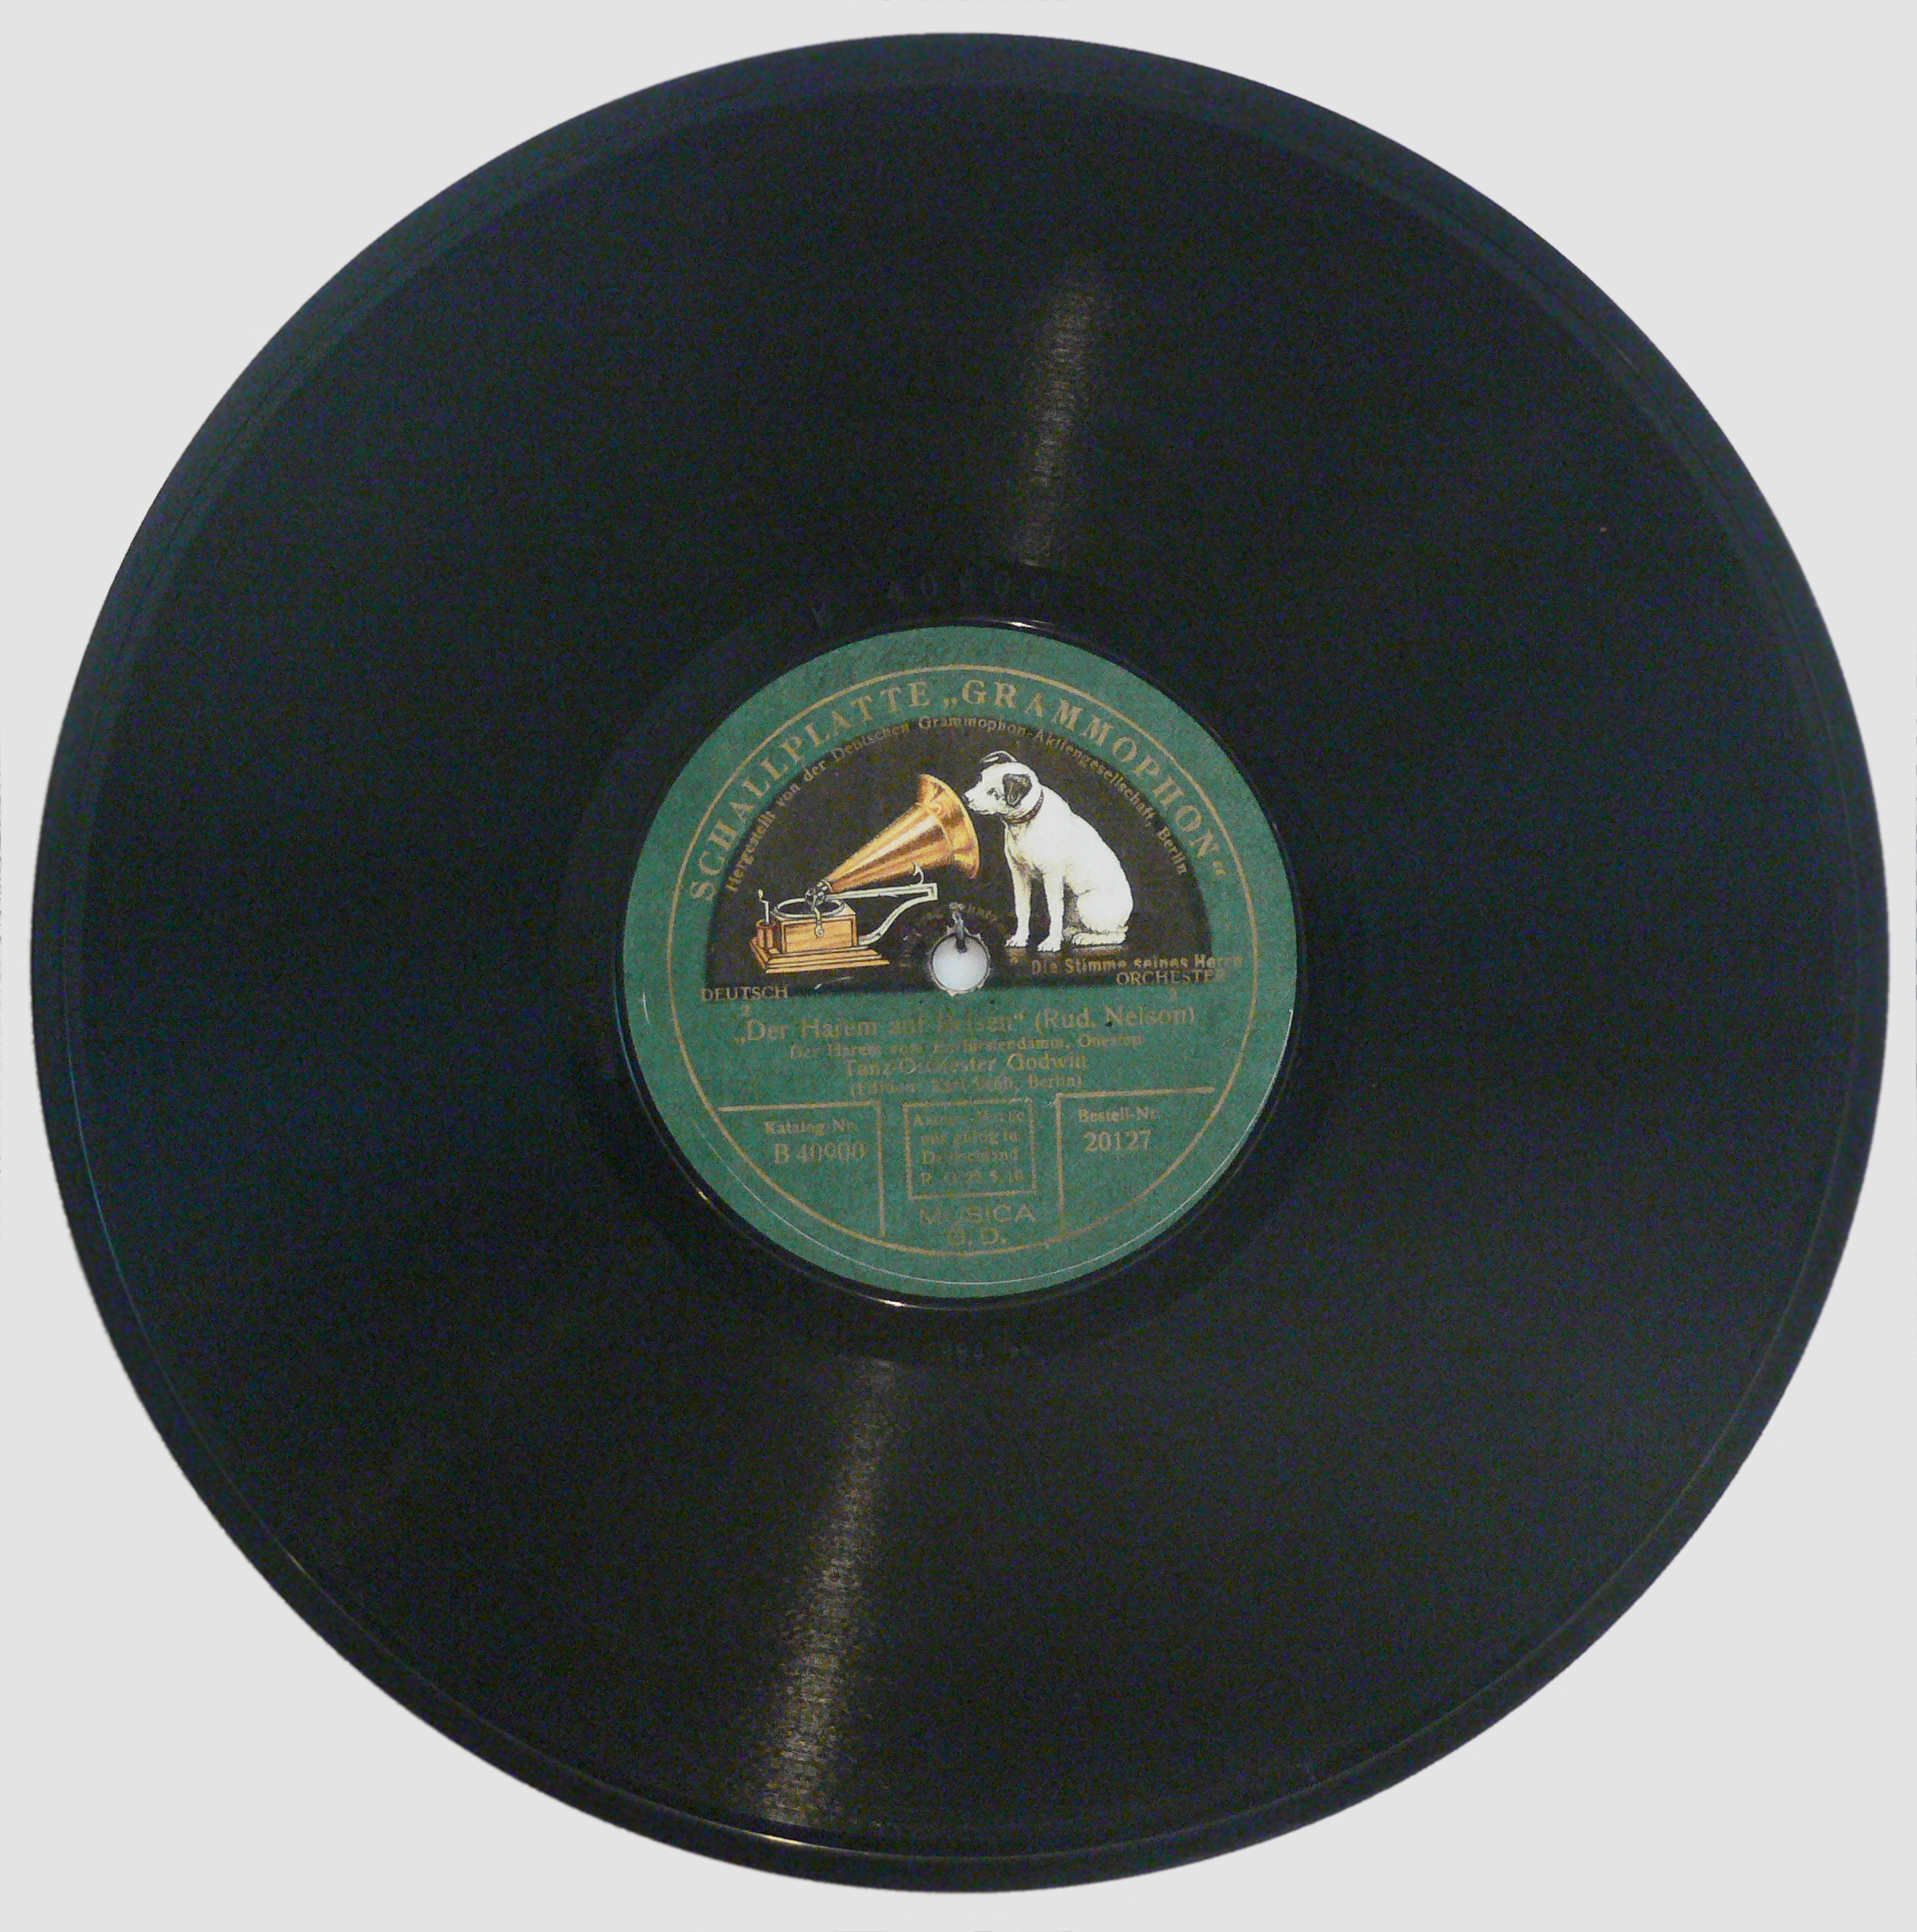
\includegraphics[height=0.1\textheight]{Bilder/Einleitung/schallplatte-schellack.png}
                    \caption[Schellackschallplatte \newline \url{https://de.wikipedia.org/wiki/Datei:Schallplatte_Deutsche_Grammophon_Stimme_seines_Herrn.jpg} (zuletzt aufgerufen am 19.09.2015)]{Schellackschall-platte}
                    \label{fig:schallplatte-schellack}
                \end{center}
            \end{minipage}
            \hspace{0.025\textwidth}
            \begin{minipage}[t]{0.3\textwidth}
                \begin{center}
                    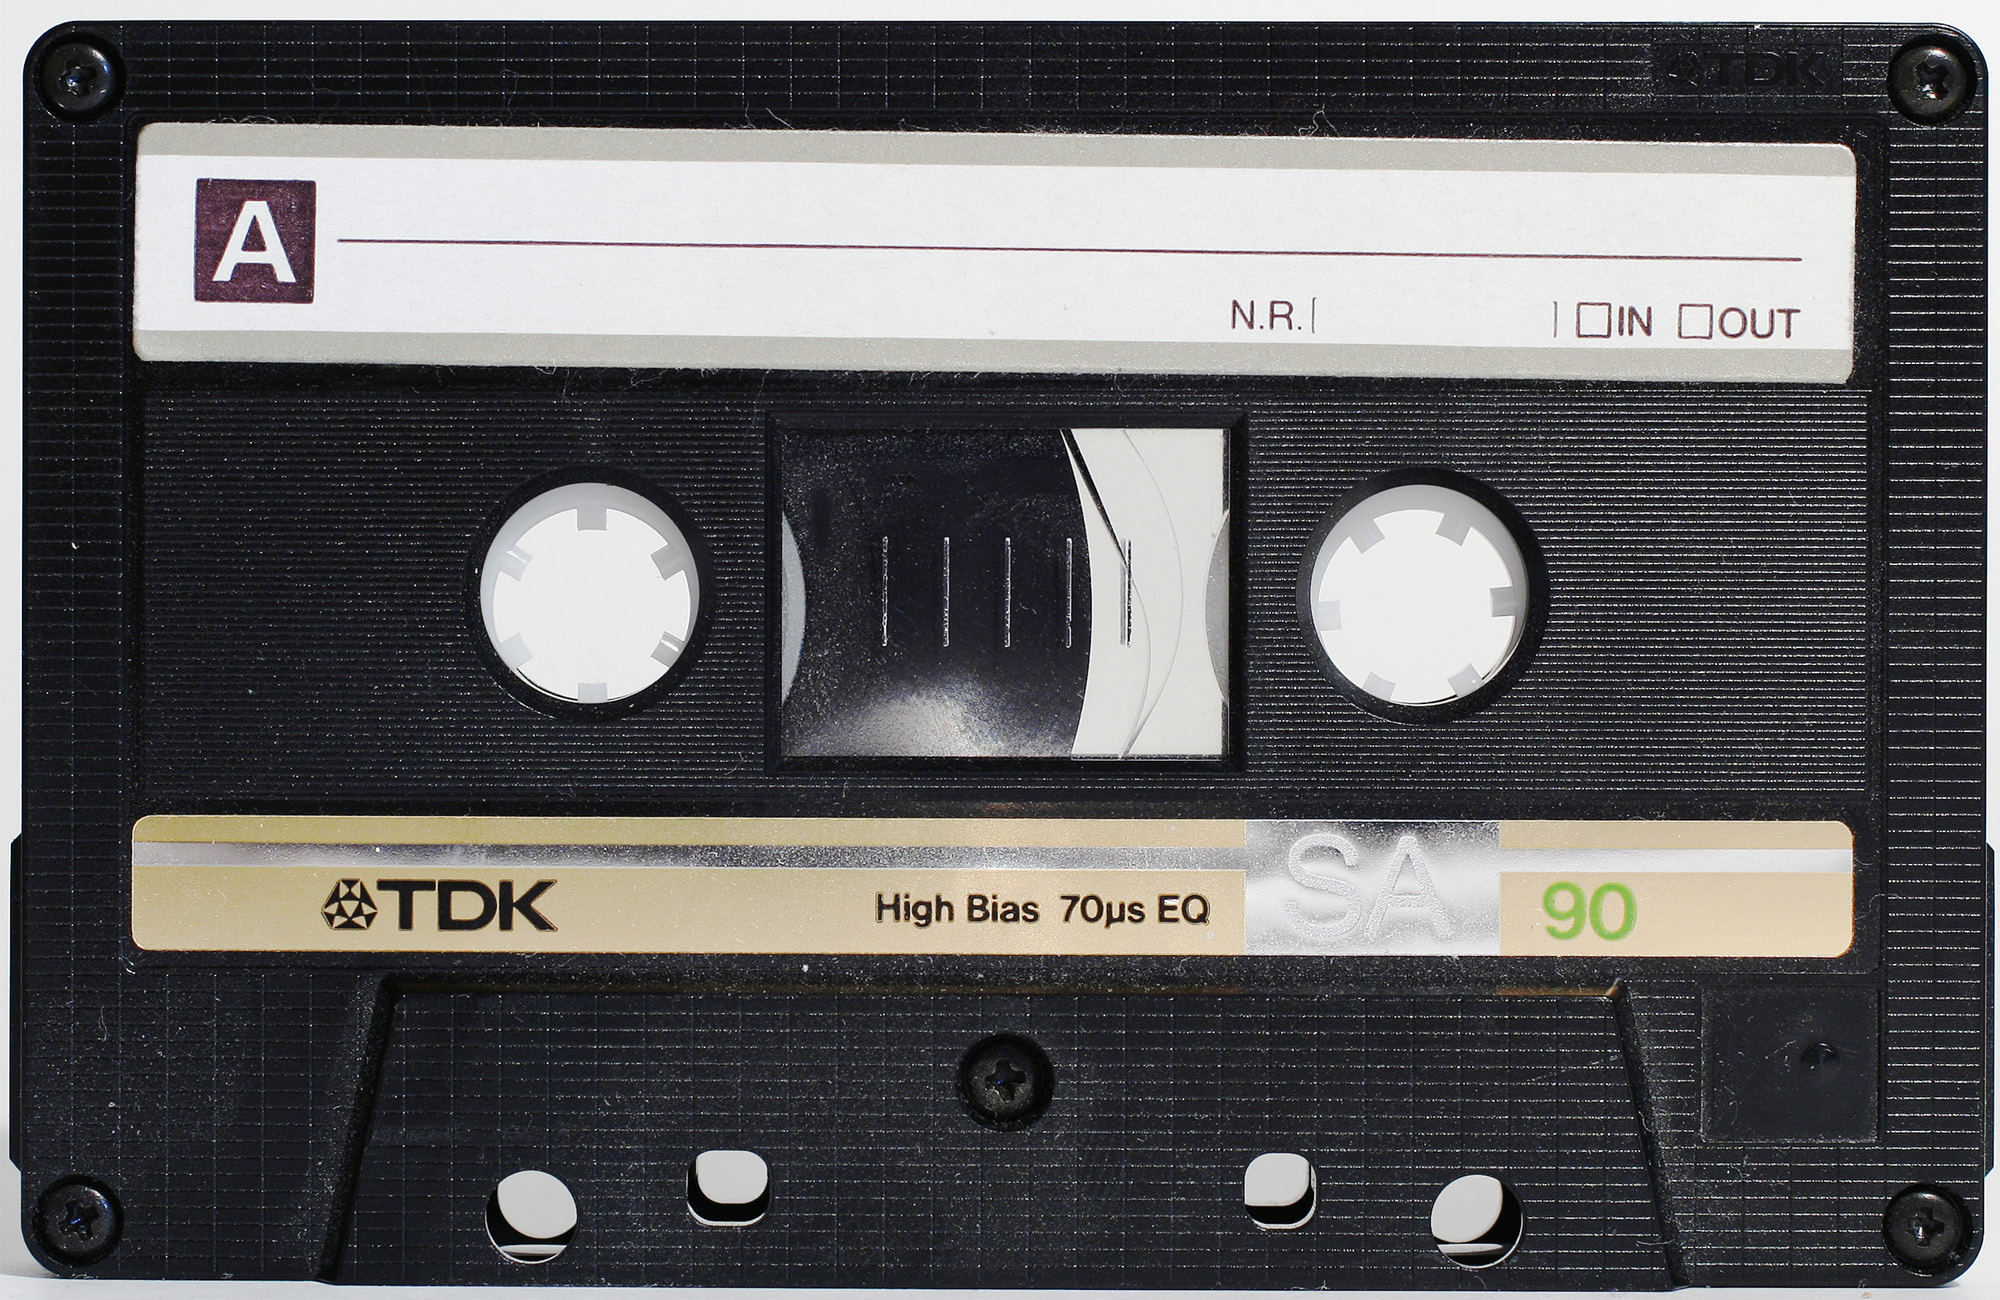
\includegraphics[height=0.1\textheight]{Bilder/Einleitung/compact-cassette.png}
                    \caption[Compact Cassette \newline \url{https://de.wikipedia.org/wiki/Datei:Compactcassette.jpg} (zuletzt aufgerufen am 19.09.2015)]{Compact Cassette}
                    \label{fig:compact-cassette}
                \end{center}
            \end{minipage}
        \end{center}
    \end{figure}
}{}

In den 80er Jahren kam die Compact Disc (CD, siehe \autoref{fig:compact-disc})
auf den Markt. Hierbei handelt es sich um einen optischen Datenträger aus dem
Kunststoff Polycarbonat handelt. Compact Discs und Digital Video Discs (DVD),
eine Weiterentwicklung der CD, zeichnen sich durch hohe Speicherkapazität sowie
geringe Abnutzungserscheinungen aus. Deshalb wurden sie zum universellen
Speichermedium für Musik, Dokumente, Bilder und Filme.

Mit der Verbreitung des Internets hat die Übertragung von Informationen mittels
Lichtsignalen in den letzten Jahren an Bedeutung gewonnen. Neben Glasfaserkabeln
werden hierfür polymer optische Fasern (POF, siehe \autoref{fig:pof})
eingesetzt.

Anhand der Beispiele der Compact Disc und der polymer optischen Faser wird in
dieser Arbeit der Einsatz von transparenten Kunststoffen in der
Informationstechnologie aufgezeigt und ihre spezielle Eignung für die
Informationsspeicherung und -weitergabe erörtert. Dabei wird auf die
Funktionsweise und Produktion von optischen Datenträgern und optischen
Wellenleitern eingegangen. Außerdem werden die physikalischen Eigenschaften und
die Herstellung der verwendeten Kunststoffe erläutert.

\ifthenelse{\boolean{showPics}}{
    \begin{figure}[h]
        \begin{center}
            \begin{minipage}[t]{0.4\textwidth}
                \begin{center}
                    \includegraphics[height=0.1\textheight]{Bilder/Einleitung/compact-disk.png}
                    \caption[Compact Disc \newline \url{https://en.wikipedia.org/wiki/File:Compact_disc.svg} (zuletzt aufgerufen am 19.09.2015)]{Compact Disc}
                    \label{fig:compact-disc}
                \end{center}
            \end{minipage}
            \hspace{0.025\textwidth}
            \begin{minipage}[t]{0.4\textwidth}
                \begin{center}
                    \includegraphics[height=0.1\textheight]{Bilder/Einleitung/pof.png}
                    \caption[polymer optische Faser \newline \url{http://www.heise.de/tr/imgs/08/2/5/4/2/1/5/c337ef89957e0f2b.jpg} (zuletzt aufgerufen am 19.09.2015)]{polymer optische Faser}
                    \label{fig:pof}
                \end{center}
            \end{minipage}
        \end{center}
    \end{figure}
}{}

\section{Optische Datenträger - Die Compact Disc}
\label{sec:cd}

\subsection{Geschichte}
\label{subsec:cdgeschichte}

Die Entwicklung von optischen Datenträgern mit einem laserbasiertem
Auslesesystem begann in den 70er Jahren des 20. Jahrhunderts. 1975 brachte
Philips den ersten optischen Datenträger auf den Markt, die Laservision
Videodisc (siehe \autoref{fig:videodisc}). Sie sollte eine Alternative zum
VHS-Videosystem (siehe \autoref{fig:vhs}) darstellen, war aufgrund geringer
Verkaufszahlen jedoch nicht erfolgreich.

\begin{figure}[h]
    \begin{center}
        \begin{minipage}[t]{0.3\textwidth}
            \begin{center}
                \includegraphics[height=0.1\textheight]{Bilder/Optische_Datentraeger_Die_Compact_Disc/Geschichte/videodisc.png}
                \caption[Laservision Videodisc \newline \url{http://www.sciencemuseum.org.uk/online_science/explore_our_collections/objects/index/smxg-8095649} (zuletzt aufgerufen am 19.09.2015)]{Laservision Videodisc}
                \label{fig:videodisc}
            \end{center}
        \end{minipage}
        \hspace{0.025\textwidth}
        \begin{minipage}[t]{0.3\textwidth}
            \begin{center}
                \includegraphics[height=0.1\textheight]{Bilder/Optische_Datentraeger_Die_Compact_Disc/Geschichte/vhs.png}
                \caption[VHS cassette \newline \url{https://upload.wikimedia.org/wikipedia/commons/6/67/VHS-cassette.jpg} (zuletzt aufgerufen am 19.09.2015)]{VHS cassette}
                \label{fig:vhs}
            \end{center}
        \end{minipage}
    \end{center}
\end{figure}

Auf Basis der Videodisc entwickelte Philips bis 1977 die Compact Disc Digital
Audio mit einem Durchmesser von 11,5 cm und einer Spielzeit von 60 Minuten.

Ab 1979 arbeiteten Philips und Sony dann an einem gemeinsamen CD-Standard. Man
einigte sich auf einen Durchmesser von 12 cm und eine 75-minütige Spielzeit.
Dieser Standard ist bis heute von allen CD-Herstellern anerkannt. \cite{cds}

Die Schallplattenproduzenten befürchteten rückläufige Verkaufszahlen. Deshalb
scheiterten die Verhandlungen betreffend die Rechte an Musikstücken für CDs.

Deshalb beschlossen Philips und Sony, sich zunächst auf klassische Musik zu
konzentrieren. Man vermutete hier einen Kundenstamm, der eher bereit wäre, für
eine bessere Klangqualität mehr Geld auszugeben.

Der CD gelang der Durchbruch während der Salzburger Festspiele im April 1981.
Philips und Sony konnten ein Publikum aus Musikkritikern von dem
Zukunftspotential der CD überzeugen. Die Begeisterung der Kritiker erfasste die
internationale Musikszene und bis März 1982 hatten acht Schallplattenfirmen
Verträge mit Philips und Sony unterschrieben. Die Markteinführung erfolgte am
17. August 1982. \cite{cuz}

Innerhalb weniger Jahre die CD verdrängte die Schallplatte fast komplett vom
Markt. \autoref{fig:umsatzcd} zeigt den Umsatz der deutschen Musikindustrie mit
den jeweiligen Produkten. Der Umsatz mit Vinylschallplatten, 1980 mit ca. 760
Mio. Euron och das umsatzstärkste Medium, sank bis 1987 erst allmählich und
dann bis 1992 rapide. Im selben Zeitraum stieg der Umsatz mit CDs massiv an und
erreichte im Jahr 1997 ein Maximum von 2,3 Mrd. Euro. Ab 1997 waren die
Verkaufszahlen rückläufig. da Privatperson selbst CDs
\shorthandoff{"}"brennen"\shorthandon{"} konnten und zunehmend legale und
illegalem Angebote im Internet nutzten.

\begin{figure}[h]
    \begin{center}
        \begin{minipage}[t]{\textwidth}
            \begin{center}
                \includegraphics[width=\textwidth]{Bilder/Optische_Datentraeger_Die_Compact_Disc/Geschichte/umsatzcd.png}
                \caption[Umsatzentwicklung der deutschen Musikindustrie \newline \url{http://www.musikindustrie.de/uploads/media/140325\_BVMI\_2013\_Jahrbuch\_ePaper\_V02.pdf} S. 7 (zuletzt aufgerufen am 03.08.2015)]{Umsatzentwicklung der deutschen Musikindustrie}
                \label{fig:umsatzcd}
            \end{center}
        \end{minipage}
    \end{center}
\end{figure}

\subsection{Funktionsweise}
\label{subsec:cdfunktionsweise}

\subsection{Herstellung der Compact Disc}
\label{subsec:cdherstellung}

Die Herstellung einer CD beginnt mit der Anfertigung einer Glasmatrize. Diese
besteht aus einer Glasplatte und einer Fotolackschicht, welche die Pitstruktur
enthält. Aus dieser wird daraufhin eine Metallmatrize gefertigt, welche für das
Spritzgussverfahren verwendet wird. Dabei wird die Matrize in das flüssige
Polycarbonat gepresst. Dadurch überträgt sich die Pitstruktur, wie in
\autoref{fig:cdherstellung}, auf die Polycarbonatscheibe. Auf diese wird
anschließend das Aluminium aufgedampft, um die Reflexionsschicht zu erhalten,
und mithilfe einer Schutzschicht versiegelt. \cite{cdp}

\begin{figure}[h]
  \begin{center}
      \begin{minipage}[t]{\textwidth}
        \begin{center}
            \includegraphics[height=0.1\textheight]{Bilder/Optische_Datentraeger_Die_Compact_Disc/Herstellung/cdherstellung.png}
            \caption[Spritzgussverfahren \newline \url{http://daten.didaktikchemie.uni-bayreuth.de/umat/cd_dvd/spritzguss.gif} (zuletzt aufgerufen am 07.08.2015)]{Spritzgussverfahren}
            \label{fig:cdherstellung}
        \end{center}
      \end{minipage}
  \end{center}
\end{figure}

%TODO: Spritzgussverfahren erklären

\subsection{Material: Polycarbonat}

\subsubsection{Vorteile von Polycarbonat gegenüber anderen Materialien}

Polycarbonat wurde 1953 von dem, bei der Firma Bayer angestellten, Chemiker
Hermann Schnell entdeckt. Der neue Kunststoff wurde später unter dem Namen
Makrolon\textsuperscript{\textregistered} vermarktet.

Nachdem seine ersten CD-Prototypen hergestellt hat, suchte man nach
Trägermaterial, welches für die Massenproduktion mittels des
Spritzgussverfahrens geeignet ist. Hierfür ist Polycarbonat nahezu perfekt. Die
niedriege Viskosität ermöglicht eine fehlerfreie übertragung der Pitstruktur von
der Matrize auf die Polycarbonatscheibe. Hohe Transparenz und ein konstater
Brechungsindex\footnote{Verhältnis der Lichtgeschwindigkeit und der
Ausbreitungsgeschwindigkeit von Licht im untersuchten Material} erlauben ein
unabgeschwächtes Durchdringen des Laserstrahls durch das Trägermaterial. Eine
hohe Erweichungstemperatur\footnote{ca. 149°C} und Resistenz gegenüber
physikalischen Belastungen machen Polycarbonat ebenfalls alltagstauglich.

Die \autoref{fig:cdpcpmma} vergleicht Polycarbonat(PC) und
Polymethylmethacrylat(PMMA) im Bezug auf Eigenschaften, die für die Herstellung
und Benutzung der CD von Vorteil sind. Die Eignung nimmt in den jeweiligen
Punkten von innen nach außen zu. PMMA schneidet in fast allen Punkten mit
Bestnote ab. Jedoch machen ein insgesamt mittelmäßiges Abschneiden von PC und
bessere Eigenschaften in den Kategorien Wärmeformbeständigkeit und geringe
Wasseraufnahme als Polymethylmethacrylat Polycarbonat zum bevorzugten Kunststoff
für die CD-Produktion.

\begin{figure}[h]
  \begin{center}
      \begin{minipage}[t]{\textwidth}
        \begin{center}
            \includegraphics[height=0.1\textheight]{Bilder/Optische_Datentraeger_Die_Compact_Disc/Material:_Polycarbonat/cdpcpmma.png}
            \caption[Vergleich zwischen PC und PMMA \newline Roth, Klaus: CD, DVD \& Co.: Die Chemie der schillernden Scheiben, in: Chemie in unserer Zeit (41/2007), S. 337]{Vergleich zwischen PC und PMMA}
            \label{fig:cdpcpmma}
        \end{center}
      \end{minipage}
  \end{center}
\end{figure}

\subsubsection{Herstellung von Polycarbonat}

Polycarbonat kann entweder über eine Umesterung oder über eine
Grenzflächenkondensation hergestellt werden. Beide Reaktionen können als
Sonderformen der Polykondensation eingeordnet werden, da ein Polyester entsteht,
sich aber kein Wasser abspaltet. Polycarbonat selbst ist ein lineares
Makromolekül und zählt somit zu den Thermoplasten, da die beiden Edukte
jeweils über zwei funktionale Gruppen verfügen.

Bei der Umesterung kommen die, in Schmelze versetzten, Monomere Bisphenol A und
Diphenylcarbonat zum Einsatz. \autoref{rec:diphenylcarbonat} zeigt die
Herstellung von Diphenylcarbonat aus Phenol und Phosgen unter Abspaltung von
Salzsäure. Bisphenol A und Diphenylcarbonat reagieren in
\autoref{rec:polycarbonat} zu Polycarbonat. Die beiden Monomere sind zu
gleichen Teilen in dem Copolymere vertreten, da sie auf alternierende Weise
angeordnet sind. Die Reaktion endet wenn keine Monomere mehr vorhanden
sind.

\begin{figure}[h]
    \begin{center}
        \footnotesize
        \setatomsep{1.7em}

        \chemname{\chemfig{*6(-=-(-OH)=-=)}}{Phenol}
        \chemsign{+}
        \chemname{\chemfig{C(=[:90]\lewis{13,O})(-[:210]\lewis{357,Cl})(-[:330]\lewis{157,Cl})}}{Phosgen}
        \chemrel{->}
        \chemname{\chemfig{C(=[:90]\lewis{13,O})(-[:210]\lewis{57,O}-[:150](*6(-=-=-=)))(-[:330]\lewis{57,O}-[:30](*6(-=-=-=)))}}{Diphenylcarbonat}
        \chemsign{+}
        \chemname{\chemfig{HCl}}{Salzsäure}

        \caption{Reaktion: Diphenylcarbonat}
        \label{rec:diphenylcarbonat}
    \end{center}
\end{figure}

\begin{figure}[h]
    \begin{center}
        \footnotesize
        \setatomsep{1.7em}

        \chemname{\chemfig{C(-[4]*6(-=-(-$\scriptstyle n$\,HO)=-=))(-[2]CH_3)(-[6]CH_3)(-[0]*6(-=-(-OH)=-=))}}{Bisphenol A}
        \chemsign{+ $\scriptstyle n$}
        \chemname{\chemfig{C(=[:90]\lewis{13,O})(-[:210]\lewis{57,O}-[:150](*6(-=-=-=)))(-[:330]\lewis{57,O}-[:30](*6(-=-=-=)))}}{Diphenylcarbonat}

        \vspace{10pt}

        \chemrel{->}
        \chemname{\chemfig{C(-[4]*6(-=-(-\lewis{26,O}-[@{op,0.75}]H)=-=))(-[2]CH_3)(-[6]CH_3)(-[0]*6(-=-(-\lewis{26,O}-C(=[2]\lewis{13,O})-[@{cl,0.75}]\lewis{26,O}-(*6(-=-=-=)))=-=))}}{Polycarbonat}
        \makebraces[23pt,23pt]{n}{op}{cl}
        \chemsign{+ $\scriptstyle (2n-1)$}
        \chemname{\chemfig{*6(-=-(-OH)=-=)}}{Phenol}

        \caption{Reaktion: Polycarbonat}
        \label{rec:polycarbonat}
    \end{center}
\end{figure}

Die \autoref{rec:deprotonierung} bis \autoref{rec:abspaltung} zeigen den ersten
Umesterungsvorgang, also den Beginn des Kettenwachstums im basischen Milieu.
Als erstes findet die Deprotonierung \autoref{rec:deprotonierung} von Bisphenol
A statt. Dabei spaltet sich ein Proton (H\textsuperscript{+}) vom einer der
Hydroxygruppen ab und lagert sich an das Hydroxidion an. Durch diesen Vorgang
wird das Bisphenol A negativ geladen und das Hydroxidion wird zu Wasser
protoniert. Die Umesterung selbst beginnt mit dem nukleophilen Angriff
\autoref{rec:nukleophilerangriff} des Bisphenol A-Anions auf das
Diphenylcarbonat. Dabei lagert sich das negativgeladene Sauerstoffatom an das
positivpolarisiertes Kohlenstoffatom des Diphenylcarbonats an. Aufgrund der
Vierbindigkeit des C-Atoms \shorthandoff{"}"klappt"\shorthandon{"} eine der
Elektronenpaarbindungen des doppeltgebunden Sauerstoffatoms zu diesem. Durch
weiteres \shorthandoff{"}"herumklappen"\shorthandon{"} von
Elektronenpaarbindungen wie in \autoref{rec:abspaltung} dargestellt ist, kann
eine der Phenylgruppen in Form eines Phenolations abgespalten werden. Dabei
bildet sich die Doppelbindung zwischen dem Sauerstoff- und dem Kohlenstoffatom
zurück und die Bindung zwischen einer der beiden Phenylgruppen und dem C-Atom
\shorthandoff{"}"klappt"\shorthandon{"} zum O-Atom. Das entstandene Carbonat
kann entweder durch eine Deprotonierung der verbliebenen Hydroxygruppe

\begin{figure}[h]
    \begin{center}
        \footnotesize
        \setatomsep{1.7em}

        \chemname{\chemfig{C(-[4]*6(-=-(-HO)=-=))(-[2]CH_3)(-[6]CH_3)(-[0]*6(-=-(-O@{pr1}H)=-=))}}{Bisphenol A}
        \chemsign{+}
        \chemname{\chemfig{@{ak1}OH(-[:135,.5,,,draw=none]\fsscrm)}}{Hydroxidion}
        \chemmove[->,shorten <=2pt]{\draw[shorten >=2pt](pr1).. controls +(90:1cm) and +(90:1cm).. (ak1);}
        \chemrel{->}
        \chemname{\chemfig{C(-[4]*6(-=-(-HO)=-=))(-[2]CH_3)(-[6]CH_3)(-[0]*6(-=-(-\lewis{026,O}(-[:45,.7,,,draw=none]\fsscrm))=-=))}}{Bisphenol A-Anion}
        \chemsign{+}
        \chemname{\chemfig{H_2O}}{Wasser}

        \caption{Reaktion: Deprotonierung}
        \label{rec:deprotonierung}
    \end{center}
\end{figure}

\begin{figure}[h]
    \begin{center}
        \footnotesize
        \setatomsep{1.7em}

        \chemname{\chemfig{C(-[4]*6(-=-(-HO)=-=))(-[2]CH_3)(-[6]CH_3)(-[0]*6(-=-(-@{np2}\lewis{026,O}(-[:45,.7,,,draw=none]\fsscrm))=-=))}}{Bisphenol A-Anion}
        \chemsign{+}
        \chemname{\chemfig{@{ep2}C(-[:25,.7,,,draw=none]\fdelp)(=[@{db2}:90]@{o2}\lewis{13,O})(-[:210]\lewis{57,O}-[:150](*6(-=-=-=)))(-[:330]\lewis{57,O}-[:30](*6(-=-=-=)))}}{Diphenylcarbonat}
        \chemmove[->,shorten <=2.5pt]{
            \draw[shorten >=2.5pt](np2).. controls +(90:1cm) and +(135:2.5cm).. (ep2);
            \draw[shorten >=6pt](db2).. controls +(0:1cm) and +(90:1cm).. (o2);}

        \vspace{10pt}

        \chemrel{->}
        \chemname{\chemfig{C(-[4]*6(-=-(-HO)=-=))(-[2]CH_3)(-[6]CH_3)(-[0]*6(-=-(-\lewis{26,O}-C(-[2]\lewis{024,O}(-[:45,.7,,,draw=none]\fsscrm))(-[0]\lewis{26,O}-(*6(=-=-=-)))(-[6]\lewis{04,O}-[6](*6(=-=-=-))))=-=))}}{}

        \caption{Reaktion: Nukleophiler Angriff}
        \label{rec:nukleophilerangriff}
    \end{center}
\end{figure}

\begin{figure}[h]
    \begin{center}
        \footnotesize
        \setatomsep{1.7em}

        \chemname{\chemfig{C(-[4]*6(-=-(-HO)=-=))(-[2]CH_3)(-[6]CH_3)(-[0]*6(-=-(-\lewis{26,O}-C(-[@{ndb3}2]@{o3}\lewis{024,O}(-[:45,.7,,,draw=none]\fsscrm))(-[0]\lewis{26,O}-(*6(=-=-=-)))(-[@{b3}6]@{p3}\lewis{04,O}-[6](*6(=-=-=-))))=-=))}}{}
        \chemmove[->,shorten <=2.5pt]{
            \draw[shorten >=2.5pt](b3).. controls +(0:1cm) and +(315:1cm).. (p3);
            \draw[shorten >=2.5pt](o3).. controls +(0:0.5cm) and +(0:0.5cm).. (ndb3);}

        \vspace{10pt}

        \chemrel{->}
        \chemnameinit{}
        \chemname{\chemfig{C(-[4]*6(-=-(-HO)=-=))(-[2]CH_3)(-[6]CH_3)(-[0]*6(-=-(-\lewis{26,O}-C(=[2]\lewis{13,O})-\lewis{26,O}-(*6(-=-=-=)))=-=))}}{Carbonat}
        \chemsign{+}
        \chemname{\chemfig{*6(-=-(-\lewis{137,O}(-[:0,.7,,,draw=none]\fsscrm))=-=)}}{Phenolation}

        \caption{Reaktion: Abspaltung eines Phenolmoleküls}
        \label{rec:abspaltung}
    \end{center}
\end{figure}

\subsubsection{Versuch: Bestätigung der hohen Lichtdurchlässigkeit von PC und der einfachen
Weiterverarbeitung}


\newpage

\section{Optische Wellenleiter - Die polymere optische Faser}

\subsection{Funktionsweise}
\label{subsec:cdfunktionsweise}

\subsection{Material: Polymethylmethacrylat}

\subsubsection{Versuch: Herstellung von Polymethylmethacrylat}
\subsubsection{Versuch: Vergleich zwischen der Synthese von Polymethylmethacrylat ohne Präpolymer und mit Präpolymer}
\label{subsubsec:versuchpmma}


\subsection{Brechzahlprofile}

\subsubsection{Stufenindexprofil (SI-POF)}

Der Stufenindex ist durchsatzschwächste Brechzahlprofil (ca. 100 Megabit/s auf
100 m, spezielle Übertragungsverfahren erlauben Bitraten im Bereich von 1
Gigabit/s). Als Kernmaterial wird Polymethylmethacrylat mit einem Durchmesser
von ca. 1 mm, welcher von einem ca. 10 µm Mantel umgeben ist, eingesetzt
\cite{pofacsi}. Altarnativ kommen auch Polystyrol und Polycarbonat zum Einsatz,
jedoch sind sie für die Datenübertragung eher ungegeignet aufgrund der
geringeren Qualität als Polymethylmethacrylat\autoref{fig:pofsi} fasst den
Aufbau und die Lichtausbreitung zusammen. Die Spalte mit Brechungsindex als
Überschrift stellt den Verlauf dieses grafisch dar. Beim Stufenindexprofil
steigen die Brechzahlen beim Übergang vom Mantel zum Kern abrupt an. Dies hat
die schon erwähnte Totalreflexion an der Kerngrenze, welche man in der Spalte
Querschnitt erkennen kann, zur Folge.

\begin{figure}[h]
    \begin{center}
        \begin{minipage}[t]{0.4\textwidth}
            \begin{center}
                \includegraphics[width=0.9\textwidth]{Bilder/Optische_Wellenleiter_Die_Polymer_Optische_Faser/Brechzahlprofile/pofsi.png}
                \caption[Aufbau des Stufenindexprofils \newline \url{http://www.itwissen.info/bilder/aufbau-und-brechungsprofil-der-stufenindex-profilfaser.png} (zuletzt aufgerufen am 19.09.2015)]{Aufbau des Stufenindexprofils}
                \label{fig:pofsi}
            \end{center}
        \end{minipage}
        \hspace{0.025\textwidth}
        \begin{minipage}[t]{0.4\textwidth}
            \begin{center}
                \includegraphics[height=0.1\textheight]{Bilder/Optische_Wellenleiter_Die_Polymer_Optische_Faser/Funktionsweise/pofdaempfung.png}
                \caption[Dämpfungsfenster bei einer polymer optischen Faser \newline \url{http://www.pofac.fh-nuernberg.de/pofac/de/was_sind_pof/images/pmma_daempfung.png} (zuletzt aufgerufen am 19.09.2015)]{Dämpfungsfenster beim Stufenprofil}
                \label{fig:pofdaempfung}
            \end{center}
        \end{minipage}
    \end{center}
\end{figure}

\autoref{fig:pofdaempfung} zeigt die Dämpfungsfenster einer polymer optischen
Faser. Diese liegen bei den Farben grün, gelb und rot. Um die Intensitätsabnahme
möglichst gering zu halten und damit die Reichweite zu erhöhen werden
Wellenlängen für die Lichtimpulse gewählt, die in den Dämpfungsfenstern liegen.
Als Lichtquelle kann zum Beispiel eine LED verwendet werden und als Empfänger
kommen Photodetektoren zum Einsatz. Der geringe Preis und die robuste
Übertragung auf kurzen Strecken machen die SI-POF zu einer beliebten alternative
gegenüber von Kupferkabeln in Industrieanlagen oder in Fahrzeugen. \cite{poflee}

\subsubsection{Gradientenindex}

Das Gradientenindexprofil bittet mit bis zu 10 Gigabit/s auf 100m deutlich
höhere Bitraten als das Stufenindexprofil. Beim Gradientenindex nimmt der
Brechungsindex vom Mantel bis zur Mitte des Kern kontinuierlich zu (siehe
\autoref{fig:pofgi} Spalte Brechungsindex). \autoref{fig:pofgi} zeigt ebenfalls
in der Spalte Längsschnitt den daraus resultierenden Lichtstrahlenverlauf.
Dieser verläuft, im Gegensatz zu der geraden Lichtausbreitung beim Stufenindex,
sinusförmig. Dadurch werden geringere Laufzeitunterschiede ermöglicht und die
Frequenz der Lichtimpulse kann erhöht werden. Außerdem wird bei der
Gradientenfaser eine Dämpfung von unter 20 dB/km erreicht (siehe
\autoref{fig:pofgidaempfung}. Dies ist ein ehrheblicher Sprung über der
Dämpfung einer Stufenfaser mit ca 100 dB/km (siehe \autoref{fig:pofdaempfung}).
Aus den beiden Gründen ist die Bandbreite einer Faser mit Gradientenindex
significant höher als die einer einer Faser mit Stufenindex. Aufgrund der hohen
Bitraten werden Gradientenfasern im \shorthandoff{"}"Local Area
Network"\shorthandon{"} (LAN) eingesetzt. Als Kernmaterial wird hier der
Kunststoff CYTOP\textsuperscript{\textregistered} der Asahi Glass Company
verwendet (siehe \autoref{subsec:pofcytop}). \cite{pofacgif}

\begin{figure}[h]
    \begin{center}
        \begin{minipage}[t]{0.4\textwidth}
            \begin{center}
                \includegraphics[height=0.1\textheight]{Bilder/Optische_Wellenleiter_Die_Polymer_Optische_Faser/Brechzahlprofile/pofgi.png}
                \caption[Aufbau des Gradientenindexprofils \newline \url{ITWissen}]{Aufbau des Gradientenindexprofils}
                \label{fig:pofgi}
            \end{center}
        \end{minipage}
        \hspace{0.025\textwidth}
        \begin{minipage}[t]{0.4\textwidth}
            \begin{center}
                \includegraphics[height=0.1\textheight]{Bilder/Optische_Wellenleiter_Die_Polymer_Optische_Faser/Brechzahlprofile/pofgidaempfung.png}
                \caption[Dämpfung bei einer Gradientenfaser \newline \url{POFAC}]{Dämpfung bei einer Gradientenfaser}
                \label{fig:pofgidaempfung}
            \end{center}
        \end{minipage}
    \end{center}
\end{figure}

%TODO: Get url


\subsection{Herstellungsverfahren}

\input{./Sections/Optische_Wellenleiter_Die_polymere_optische_Faser/Herstellungsverfahren/Aetzverfahren}
\input{./Sections/Optische_Wellenleiter_Die_polymere_optische_Faser/Herstellungsverfahren/Replikationsverfahren}
\input{./Sections/Optische_Wellenleiter_Die_polymere_optische_Faser/Herstellungsverfahren/Fotochemische_Strukturierung}

\subsection{Vergleich zur Glasfaser}
\label{subsec:pofglasfaser}

\section{Fazit}
\label{sec:schluss}

Transparente Kunststoffe sind auch zukünftig aus der Informationstechnologie
nicht wegzudenken. Optische Datenträger werden zwar an Bedeutung verlieren: so
prognostiziert der Bundesverband Musikindustrie e.V. für physische Tonträger
(CD, DVD, ...) einen Umsatzrückgang von 1,1 Mrd. \euro{} im Jahr 2013 auf 800
Mio. \euro{} im Jahr 2018 (\autoref{fig:umsatzprog}). Jedoch werden
Musikangebote über das Internet (Downloadportale und Streaming-Angebote) an
Bedeutung gewinnen: bis 2018 wird der Anteil der Internetangebote am
Gesamtumsatz von \nolbreaks{23 \%} in 2013 auf \nolbreaks{50 \%} steigen und
damit gleichauf mit dem Umsatzanteil von physischen Datenträgern liegen.

\ifthenelse{\boolean{showPics}}{
    \begin{figure}[h]
        \begin{center}
            \begin{minipage}[t]{\textwidth}
                \begin{center}
                    \includegraphics[width=\textwidth]{Bilder/Schluss/prognose.png}
                    \caption[Prognose für die Umsatzanteile in der Musikindustrie bis 2018 \newline verändert nach \url{http://www.musikindustrie.de/uploads/media/140325\_BVMI\_2013\_Jahrbuch\_ePaper\_V02.pdf} S.15 \newline (zuletzt aufgerufen am 03.08.2015)]{Prognose für die Umsatzanteile in der Musikindustrie bis 2018}
                    \label{fig:umsatzprog}
                \end{center}
            \end{minipage}
        \end{center}
    \end{figure}
}{}

Internetangebote werden aber auch für die Film- und Fernsehindustrie immer
wichtiger: viele Sender betreiben Mediatheken mit den aktuellen
Fernsehsendungen; statt eine DVD oder Blue-Ray-Disc zu kaufen oder auszuleihen
werden Filme aus Videoportalen wie Maxdome und Amazon Prime geladen; Netflix
bietet Serien und Filme ausschließlich online an.

Um bei hochauflösenden Filmen lange Wartezeiten und \glqq Ruckler\grqq{} zu
vermeiden, sind hohe Übertragungsraten auch für Privathaushalte notwendig. Diese
Bandbreiten werden u.a. erreicht, indem Privathaushalte über Kabel aus polymer
optischen Fasern an Glasfasernetze angeschlossen werden.

Somit geht mit dem Bedeutungsverlust optischer Datenträger die zunehmende
Verbreitung optischer Wellenleiter einher.


\begin{thebibliography}{99}

\bibitem{schallplatte1}{UNI-Protokolle: Schallplatte, zuletzt aufgerufen am 01.07.2015 \newline
\url{http://www.uni-protokolle.de/Lexikon/Schallplatte.html}}

\bibitem{kassette1}{UNI-Protokolle: Tonband, zuletzt aufgerufen am 01.07.2015 \newline
\url{http://www.uni-protokolle.de/Lexikon/Tonband.html}}

\bibitem{kassette2}{Tonaufzeichnung damals \& heute: Compact-Cassette: Ein Renner vor allem bei
Kindern, zuletzt aufgerufen am 01.07.2015 \newline
\url{http://www.tonaufzeichnung.de/medien/compactcassette}}

\bibitem{cd_durchbruch}{Bundesverband Musikindustrie: Musikindustrie in Zahlen, S. 7, zuletzt
aufgerufen am 01.07.2015 \newline
\url{http://www.musikindustrie.de/uploads/media/140325\_BVMI\_2013\_Jahrbuch\_ePaper\_V02.pdf}}

\end{thebibliography}

\end{document}
